\documentclass[twoside]{book}

% Packages required by doxygen
\usepackage{calc}
\usepackage{doxygen}
\usepackage{graphicx}
\usepackage[utf8]{inputenc}
\usepackage{makeidx}
\usepackage{multicol}
\usepackage{multirow}
\usepackage{textcomp}
\usepackage[table]{xcolor}

% Font selection
\usepackage[T1]{fontenc}
\usepackage{mathptmx}
\usepackage[scaled=.90]{helvet}
\usepackage{courier}
\usepackage{amssymb}
\usepackage{sectsty}
\renewcommand{\familydefault}{\sfdefault}
\allsectionsfont{%
  \fontseries{bc}\selectfont%
  \color{darkgray}%
}
\renewcommand{\DoxyLabelFont}{%
  \fontseries{bc}\selectfont%
  \color{darkgray}%
}

% Page & text layout
\usepackage{geometry}
\geometry{%
  a4paper,%
  top=2.5cm,%
  bottom=2.5cm,%
  left=2.5cm,%
  right=2.5cm%
}
\tolerance=750
\hfuzz=15pt
\hbadness=750
\setlength{\emergencystretch}{15pt}
\setlength{\parindent}{0cm}
\setlength{\parskip}{0.2cm}
\makeatletter
\renewcommand{\paragraph}{%
  \@startsection{paragraph}{4}{0ex}{-1.0ex}{1.0ex}{%
    \normalfont\normalsize\bfseries\SS@parafont%
  }%
}
\renewcommand{\subparagraph}{%
  \@startsection{subparagraph}{5}{0ex}{-1.0ex}{1.0ex}{%
    \normalfont\normalsize\bfseries\SS@subparafont%
  }%
}
\makeatother

% Headers & footers
\usepackage{fancyhdr}
\pagestyle{fancyplain}
\fancyhead[LE]{\fancyplain{}{\bfseries\thepage}}
\fancyhead[CE]{\fancyplain{}{}}
\fancyhead[RE]{\fancyplain{}{\bfseries\leftmark}}
\fancyhead[LO]{\fancyplain{}{\bfseries\rightmark}}
\fancyhead[CO]{\fancyplain{}{}}
\fancyhead[RO]{\fancyplain{}{\bfseries\thepage}}
\fancyfoot[LE]{\fancyplain{}{}}
\fancyfoot[CE]{\fancyplain{}{}}
\fancyfoot[RE]{\fancyplain{}{\bfseries\scriptsize Generated on Mon May 9 2016 21\-:31\-:16 for My Project by Doxygen }}
\fancyfoot[LO]{\fancyplain{}{\bfseries\scriptsize Generated on Mon May 9 2016 21\-:31\-:16 for My Project by Doxygen }}
\fancyfoot[CO]{\fancyplain{}{}}
\fancyfoot[RO]{\fancyplain{}{}}
\renewcommand{\footrulewidth}{0.4pt}
\renewcommand{\chaptermark}[1]{%
  \markboth{#1}{}%
}
\renewcommand{\sectionmark}[1]{%
  \markright{\thesection\ #1}%
}

% Indices & bibliography
\usepackage{natbib}
\usepackage[titles]{tocloft}
\setcounter{tocdepth}{3}
\setcounter{secnumdepth}{5}
\makeindex

% Hyperlinks (required, but should be loaded last)
\usepackage{ifpdf}
\ifpdf
  \usepackage[pdftex,pagebackref=true]{hyperref}
\else
  \usepackage[ps2pdf,pagebackref=true]{hyperref}
\fi
\hypersetup{%
  colorlinks=true,%
  linkcolor=blue,%
  citecolor=blue,%
  unicode%
}

% Custom commands
\newcommand{\clearemptydoublepage}{%
  \newpage{\pagestyle{empty}\cleardoublepage}%
}


%===== C O N T E N T S =====

\begin{document}

% Titlepage & ToC
\hypersetup{pageanchor=false}
\pagenumbering{roman}
\begin{titlepage}
\vspace*{7cm}
\begin{center}%
{\Large My Project }\\
\vspace*{1cm}
{\large Generated by Doxygen 1.8.6}\\
\vspace*{0.5cm}
{\small Mon May 9 2016 21:31:16}\\
\end{center}
\end{titlepage}
\clearemptydoublepage
\tableofcontents
\clearemptydoublepage
\pagenumbering{arabic}
\hypersetup{pageanchor=true}

%--- Begin generated contents ---
\chapter{Hierarchical Index}
\section{Class Hierarchy}
This inheritance list is sorted roughly, but not completely, alphabetically\-:\begin{DoxyCompactList}
\item \contentsline{section}{Character}{\pageref{class_character}}{}
\begin{DoxyCompactList}
\item \contentsline{section}{Bad}{\pageref{class_bad}}{}
\item \contentsline{section}{Good}{\pageref{class_good}}{}
\item \contentsline{section}{Zombie}{\pageref{class_zombie}}{}
\end{DoxyCompactList}
\item exception\begin{DoxyCompactList}
\item \contentsline{section}{Unrecognized\-Character\-Exception}{\pageref{class_unrecognized_character_exception}}{}
\item \contentsline{section}{Unrecognized\-Conversion\-Exception}{\pageref{class_unrecognized_conversion_exception}}{}
\end{DoxyCompactList}
\item \contentsline{section}{Person}{\pageref{class_person}}{}
\item \contentsline{section}{World}{\pageref{class_world}}{}
\end{DoxyCompactList}

\chapter{Class Index}
\section{Class List}
Here are the classes, structs, unions and interfaces with brief descriptions\-:\begin{DoxyCompactList}
\item\contentsline{section}{\hyperlink{class_bad}{Bad} }{\pageref{class_bad}}{}
\item\contentsline{section}{\hyperlink{class_character}{Character} }{\pageref{class_character}}{}
\item\contentsline{section}{\hyperlink{class_good}{Good} }{\pageref{class_good}}{}
\item\contentsline{section}{\hyperlink{class_person}{Person} }{\pageref{class_person}}{}
\item\contentsline{section}{\hyperlink{class_unrecognized_character_exception}{Unrecognized\-Character\-Exception} }{\pageref{class_unrecognized_character_exception}}{}
\item\contentsline{section}{\hyperlink{class_unrecognized_conversion_exception}{Unrecognized\-Conversion\-Exception} }{\pageref{class_unrecognized_conversion_exception}}{}
\item\contentsline{section}{\hyperlink{class_world}{World} }{\pageref{class_world}}{}
\item\contentsline{section}{\hyperlink{class_zombie}{Zombie} }{\pageref{class_zombie}}{}
\end{DoxyCompactList}

\chapter{Class Documentation}
\hypertarget{class_bad}{\section{Bad Class Reference}
\label{class_bad}\index{Bad@{Bad}}
}


Inheritance diagram for Bad\-:
\nopagebreak
\begin{figure}[H]
\begin{center}
\leavevmode
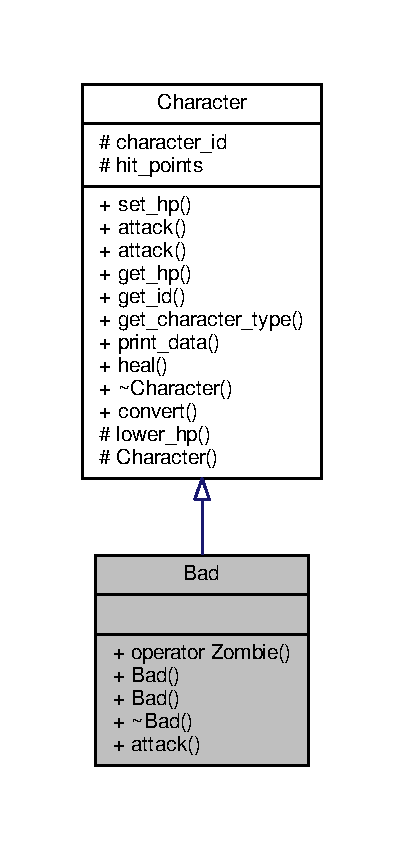
\includegraphics[width=194pt]{class_bad__inherit__graph}
\end{center}
\end{figure}


Collaboration diagram for Bad\-:
\nopagebreak
\begin{figure}[H]
\begin{center}
\leavevmode
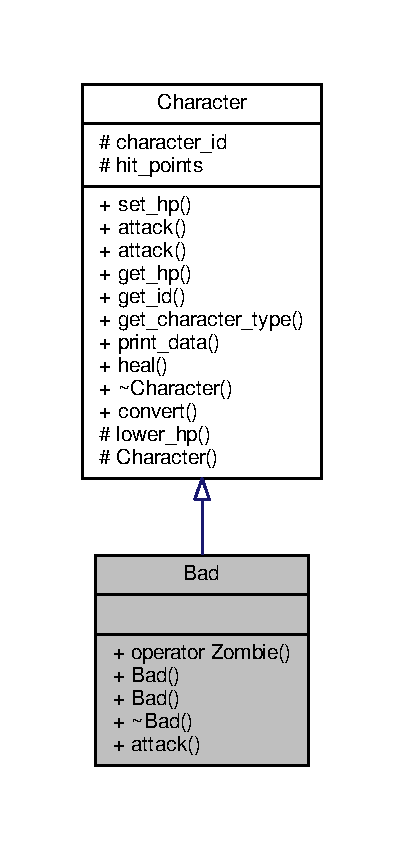
\includegraphics[width=194pt]{class_bad__coll__graph}
\end{center}
\end{figure}
\subsection*{Public Member Functions}
\begin{DoxyCompactItemize}
\item 
\hyperlink{class_bad_a788976f950638afe79e2d8dbff20fb3d}{operator Zombie} ()
\item 
\hypertarget{class_bad_ac3ce1c334b89717956276e94e496d068}{{\bfseries Bad} (\hyperlink{class_character}{Character} \&)}\label{class_bad_ac3ce1c334b89717956276e94e496d068}

\item 
\hypertarget{class_bad_ad2e8efaa0a84262c5983367e95fb8a3d}{\hyperlink{class_person}{Person} $\ast$ {\bfseries attack} (\hyperlink{class_person}{Person} $\ast$)}\label{class_bad_ad2e8efaa0a84262c5983367e95fb8a3d}

\end{DoxyCompactItemize}
\subsection*{Additional Inherited Members}


\subsection{Member Function Documentation}
\hypertarget{class_bad_a788976f950638afe79e2d8dbff20fb3d}{\index{Bad@{Bad}!operator Zombie@{operator Zombie}}
\index{operator Zombie@{operator Zombie}!Bad@{Bad}}
\subsubsection[{operator Zombie}]{\setlength{\rightskip}{0pt plus 5cm}Bad\-::operator {\bf Zombie} (
\begin{DoxyParamCaption}
{}
\end{DoxyParamCaption}
)}}\label{class_bad_a788976f950638afe79e2d8dbff20fb3d}
This class inherits from \hyperlink{class_character}{Character} and is used to create \hyperlink{class_bad}{Bad} Characters 

The documentation for this class was generated from the following files\-:\begin{DoxyCompactItemize}
\item 
characters.\-h\item 
characters.\-cpp\end{DoxyCompactItemize}

\hypertarget{class_character}{\section{Character Class Reference}
\label{class_character}\index{Character@{Character}}
}


Inheritance diagram for Character\-:
\nopagebreak
\begin{figure}[H]
\begin{center}
\leavevmode
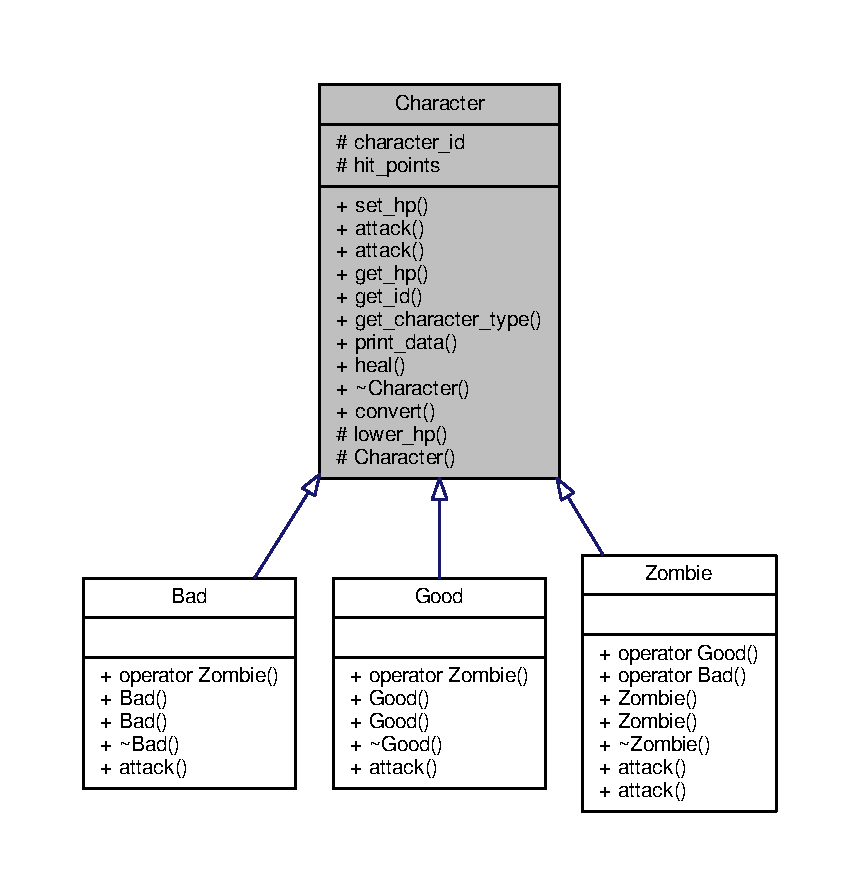
\includegraphics[width=350pt]{class_character__inherit__graph}
\end{center}
\end{figure}


Collaboration diagram for Character\-:
\nopagebreak
\begin{figure}[H]
\begin{center}
\leavevmode
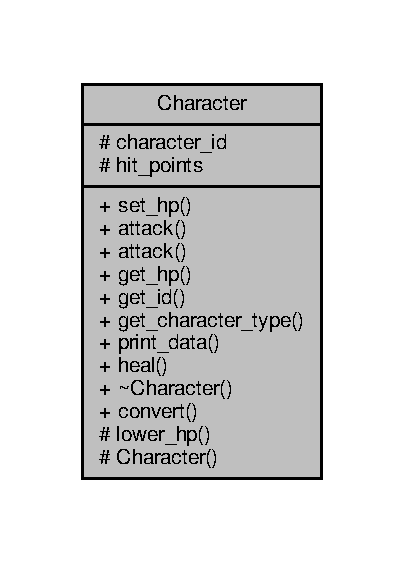
\includegraphics[width=194pt]{class_character__coll__graph}
\end{center}
\end{figure}
\subsection*{Public Member Functions}
\begin{DoxyCompactItemize}
\item 
\hypertarget{class_character_a94c3b14ee3f87d9740a12dba0eb65534}{void {\bfseries set\-\_\-hp} (int hp)}\label{class_character_a94c3b14ee3f87d9740a12dba0eb65534}

\item 
\hypertarget{class_character_a8ae210154a514c5c6c0a5dbfb5cbf8db}{virtual \hyperlink{class_character}{Character} $\ast$ {\bfseries attack} (\hyperlink{class_character}{Character} \&)}\label{class_character_a8ae210154a514c5c6c0a5dbfb5cbf8db}

\item 
\hypertarget{class_character_ae76d4df2c954ffdf55ef73560c778950}{virtual \hyperlink{class_person}{Person} $\ast$ {\bfseries attack} (\hyperlink{class_person}{Person} $\ast$)}\label{class_character_ae76d4df2c954ffdf55ef73560c778950}

\item 
\hypertarget{class_character_a39658f9ea6c4f6bc8330a73b9ea6177b}{virtual int {\bfseries get\-\_\-hp} ()}\label{class_character_a39658f9ea6c4f6bc8330a73b9ea6177b}

\item 
\hypertarget{class_character_a43b86db76f3c3f2c320c1122848f9bd8}{virtual int {\bfseries get\-\_\-id} ()}\label{class_character_a43b86db76f3c3f2c320c1122848f9bd8}

\item 
\hypertarget{class_character_afcf8a07ca3e5cd4af6d05fae7b0edff9}{virtual char $\ast$ {\bfseries get\-\_\-character\-\_\-type} ()}\label{class_character_afcf8a07ca3e5cd4af6d05fae7b0edff9}

\item 
\hypertarget{class_character_a4e86af41dea9b5422b90f3abcd09efc6}{void {\bfseries print\-\_\-data} ()}\label{class_character_a4e86af41dea9b5422b90f3abcd09efc6}

\item 
\hypertarget{class_character_a3871907535bb9cf3a042822e2dd1ec5c}{virtual void {\bfseries heal} ()}\label{class_character_a3871907535bb9cf3a042822e2dd1ec5c}

\item 
\hypertarget{class_character_a00f45ae6f4660427482165ddc1e7c792}{\hyperlink{class_character}{Character} \& {\bfseries convert} (Player\-Type T)}\label{class_character_a00f45ae6f4660427482165ddc1e7c792}

\end{DoxyCompactItemize}
\subsection*{Protected Member Functions}
\begin{DoxyCompactItemize}
\item 
\hypertarget{class_character_af859d7b80d7041535c55625ee8606a53}{void {\bfseries lower\-\_\-hp} (int)}\label{class_character_af859d7b80d7041535c55625ee8606a53}

\item 
\hypertarget{class_character_a48a3d7d8b856d6fc9d121b55f3b5acbd}{{\bfseries Character} (Player\-Type id)}\label{class_character_a48a3d7d8b856d6fc9d121b55f3b5acbd}

\end{DoxyCompactItemize}
\subsection*{Protected Attributes}
\begin{DoxyCompactItemize}
\item 
\hypertarget{class_character_a04a4d9685422d045c9069fc0defb018c}{Player\-Type {\bfseries character\-\_\-id}}\label{class_character_a04a4d9685422d045c9069fc0defb018c}

\item 
\hypertarget{class_character_a377ee5a771148b279410d5e009b8fdb7}{unsigned int {\bfseries hit\-\_\-points}}\label{class_character_a377ee5a771148b279410d5e009b8fdb7}

\end{DoxyCompactItemize}
\subsection*{Friends}
\begin{DoxyCompactItemize}
\item 
\hypertarget{class_character_a32c4cbc64da4f589025482133657589e}{class {\bfseries Zombie}}\label{class_character_a32c4cbc64da4f589025482133657589e}

\item 
\hypertarget{class_character_a3746da06cf8650489c4321e2a0022743}{class {\bfseries Good}}\label{class_character_a3746da06cf8650489c4321e2a0022743}

\item 
\hypertarget{class_character_aebdac9a0d6fcff47d9941dff13c911e6}{class {\bfseries Bad}}\label{class_character_aebdac9a0d6fcff47d9941dff13c911e6}

\item 
\hypertarget{class_character_a4f3ed79e13d2ed83c864a5f03626c4ff}{class {\bfseries Person}}\label{class_character_a4f3ed79e13d2ed83c864a5f03626c4ff}

\item 
\hypertarget{class_character_a7b4bcdf992c21ae83363f25df05b1d25}{class {\bfseries World}}\label{class_character_a7b4bcdf992c21ae83363f25df05b1d25}

\item 
\hypertarget{class_character_af456b5f771ae803ac2f56c8b7efe743c}{\hyperlink{class_character}{Character} $\ast$ {\bfseries convert\-\_\-to} (\hyperlink{class_character}{Character} $\ast$, Player\-Type)}\label{class_character_af456b5f771ae803ac2f56c8b7efe743c}

\end{DoxyCompactItemize}


The documentation for this class was generated from the following files\-:\begin{DoxyCompactItemize}
\item 
characters.\-h\item 
characters.\-cpp\item 
world.\-cpp\end{DoxyCompactItemize}

\hypertarget{class_good}{\section{Good Class Reference}
\label{class_good}\index{Good@{Good}}
}


Inheritance diagram for Good\-:
\nopagebreak
\begin{figure}[H]
\begin{center}
\leavevmode
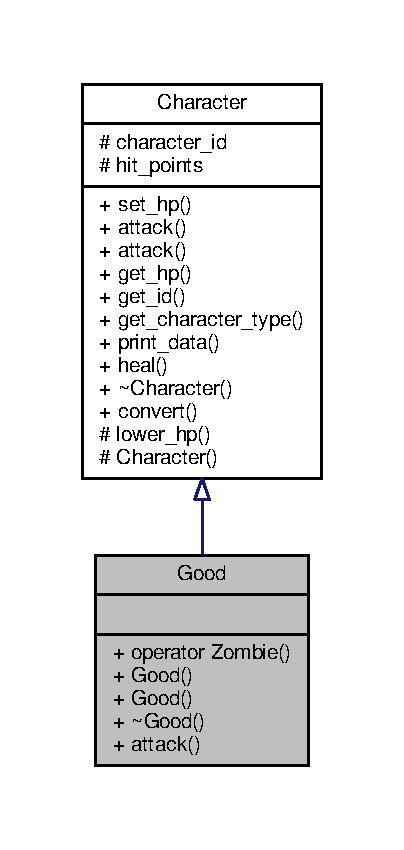
\includegraphics[width=194pt]{class_good__inherit__graph}
\end{center}
\end{figure}


Collaboration diagram for Good\-:
\nopagebreak
\begin{figure}[H]
\begin{center}
\leavevmode
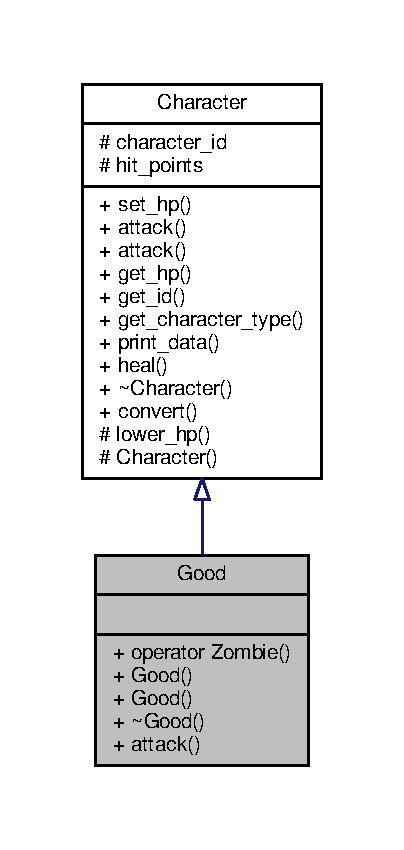
\includegraphics[width=194pt]{class_good__coll__graph}
\end{center}
\end{figure}
\subsection*{Public Member Functions}
\begin{DoxyCompactItemize}
\item 
\hyperlink{class_good_aa1e17337318e0a5a31e1168fb50a4431}{operator Zombie} ()
\item 
\hypertarget{class_good_a3038817bf388a0cab7a7ca142df1e26a}{{\bfseries Good} (\hyperlink{class_character}{Character} \&)}\label{class_good_a3038817bf388a0cab7a7ca142df1e26a}

\item 
\hypertarget{class_good_afee476ad676960b4ab2f18685c514f36}{\hyperlink{class_person}{Person} $\ast$ {\bfseries attack} (\hyperlink{class_person}{Person} $\ast$)}\label{class_good_afee476ad676960b4ab2f18685c514f36}

\end{DoxyCompactItemize}
\subsection*{Additional Inherited Members}


\subsection{Member Function Documentation}
\hypertarget{class_good_aa1e17337318e0a5a31e1168fb50a4431}{\index{Good@{Good}!operator Zombie@{operator Zombie}}
\index{operator Zombie@{operator Zombie}!Good@{Good}}
\subsubsection[{operator Zombie}]{\setlength{\rightskip}{0pt plus 5cm}Good\-::operator {\bf Zombie} (
\begin{DoxyParamCaption}
{}
\end{DoxyParamCaption}
)}}\label{class_good_aa1e17337318e0a5a31e1168fb50a4431}
This class inherits from \hyperlink{class_character}{Character} and is used to create \hyperlink{class_good}{Good} Characters 

The documentation for this class was generated from the following files\-:\begin{DoxyCompactItemize}
\item 
characters.\-h\item 
characters.\-cpp\end{DoxyCompactItemize}

\hypertarget{class_person}{\section{Person Class Reference}
\label{class_person}\index{Person@{Person}}
}


Collaboration diagram for Person\-:
\nopagebreak
\begin{figure}[H]
\begin{center}
\leavevmode
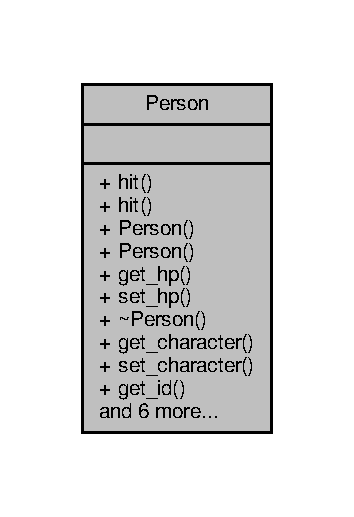
\includegraphics[width=170pt]{class_person__coll__graph}
\end{center}
\end{figure}
\subsection*{Public Member Functions}
\begin{DoxyCompactItemize}
\item 
\hypertarget{class_person_a63ead3adb6beeedcadc0b12adbf436d4}{\hyperlink{class_character}{Character} $\ast$ {\bfseries hit} (\hyperlink{class_character}{Character} $\ast$)}\label{class_person_a63ead3adb6beeedcadc0b12adbf436d4}

\item 
\hypertarget{class_person_a996677bde06c69e7f37a9c504ae8ea09}{\hyperlink{class_person}{Person} $\ast$ {\bfseries hit} (\hyperlink{class_person}{Person} $\ast$)}\label{class_person_a996677bde06c69e7f37a9c504ae8ea09}

\item 
\hypertarget{class_person_a3a60d3f9aa1025447ab4a3591275d6c3}{{\bfseries Person} (\hyperlink{class_character}{Character} $\ast$)}\label{class_person_a3a60d3f9aa1025447ab4a3591275d6c3}

\item 
\hypertarget{class_person_ac31ec51569cb94e99e35369b5f3a9f4e}{{\bfseries Person} (Player\-Type, bool)}\label{class_person_ac31ec51569cb94e99e35369b5f3a9f4e}

\item 
\hypertarget{class_person_ae18757c3ea26b6476a3f411312620c56}{int {\bfseries get\-\_\-hp} ()}\label{class_person_ae18757c3ea26b6476a3f411312620c56}

\item 
\hypertarget{class_person_a461b44c0d259b68793e26f882b526721}{void {\bfseries set\-\_\-hp} (int)}\label{class_person_a461b44c0d259b68793e26f882b526721}

\item 
\hypertarget{class_person_ae31f5b9288af821ac8bf28fffd5894ee}{\hyperlink{class_character}{Character} $\ast$ {\bfseries get\-\_\-character} ()}\label{class_person_ae31f5b9288af821ac8bf28fffd5894ee}

\item 
\hypertarget{class_person_a3bdeadc2ca985375a6446a72e497ed7d}{void {\bfseries set\-\_\-character} (\hyperlink{class_character}{Character} $\ast$)}\label{class_person_a3bdeadc2ca985375a6446a72e497ed7d}

\item 
\hypertarget{class_person_a94f3b09f82503b4eb8d701b0d0637238}{Player\-Type {\bfseries get\-\_\-id} ()}\label{class_person_a94f3b09f82503b4eb8d701b0d0637238}

\item 
\hypertarget{class_person_a1be820461df77d05bc9205ed9a304a84}{\hyperlink{class_character}{Character} $\ast$ {\bfseries convert} (Player\-Type)}\label{class_person_a1be820461df77d05bc9205ed9a304a84}

\item 
\hypertarget{class_person_aad0dd929eebdfd78cf6d99bdd792dd36}{void {\bfseries lower\-\_\-hp} ()}\label{class_person_aad0dd929eebdfd78cf6d99bdd792dd36}

\item 
\hypertarget{class_person_a2a81a35e2a6c15b5ac8787f64e1531f0}{void {\bfseries heal} ()}\label{class_person_a2a81a35e2a6c15b5ac8787f64e1531f0}

\item 
\hypertarget{class_person_aa43d99ab6de143fa6ee2bae94e25de92}{void {\bfseries print\-\_\-data} ()}\label{class_person_aa43d99ab6de143fa6ee2bae94e25de92}

\item 
\hypertarget{class_person_a2eeddf35fd72feda9ee79cb97cf4c77b}{\hyperlink{class_character}{Character} $\ast$ {\bfseries get\-\_\-attached\-\_\-character} ()}\label{class_person_a2eeddf35fd72feda9ee79cb97cf4c77b}

\item 
\hypertarget{class_person_ada0d3926855edff9375c100d118ad497}{void {\bfseries set\-\_\-attached\-\_\-character} (\hyperlink{class_character}{Character} $\ast$)}\label{class_person_ada0d3926855edff9375c100d118ad497}

\end{DoxyCompactItemize}
\subsection*{Friends}
\begin{DoxyCompactItemize}
\item 
\hypertarget{class_person_aad4eb6c63c6ff5e1ec0a11439ec421ad}{\hyperlink{class_person}{Person} $\ast$ {\bfseries convert\-\_\-to} (\hyperlink{class_person}{Person} $\ast$, Player\-Type)}\label{class_person_aad4eb6c63c6ff5e1ec0a11439ec421ad}

\end{DoxyCompactItemize}


The documentation for this class was generated from the following files\-:\begin{DoxyCompactItemize}
\item 
characters.\-h\item 
characters.\-cpp\item 
world.\-cpp\end{DoxyCompactItemize}

\hypertarget{class_unrecognized_character_exception}{\section{Unrecognized\-Character\-Exception Class Reference}
\label{class_unrecognized_character_exception}\index{Unrecognized\-Character\-Exception@{Unrecognized\-Character\-Exception}}
}


Inheritance diagram for Unrecognized\-Character\-Exception\-:
\nopagebreak
\begin{figure}[H]
\begin{center}
\leavevmode
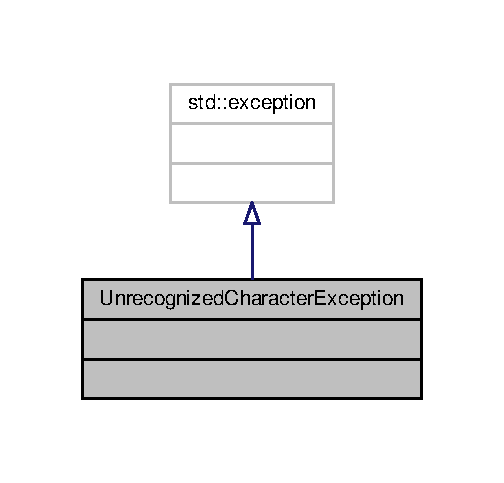
\includegraphics[width=242pt]{class_unrecognized_character_exception__inherit__graph}
\end{center}
\end{figure}


Collaboration diagram for Unrecognized\-Character\-Exception\-:
\nopagebreak
\begin{figure}[H]
\begin{center}
\leavevmode
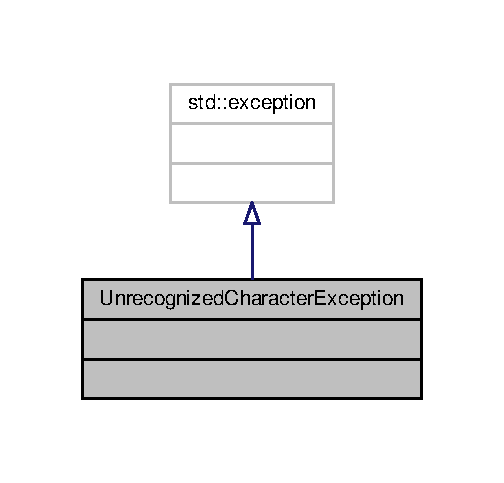
\includegraphics[width=242pt]{class_unrecognized_character_exception__coll__graph}
\end{center}
\end{figure}


The documentation for this class was generated from the following file\-:\begin{DoxyCompactItemize}
\item 
characters.\-h\end{DoxyCompactItemize}

\hypertarget{class_unrecognized_conversion_exception}{\section{Unrecognized\-Conversion\-Exception Class Reference}
\label{class_unrecognized_conversion_exception}\index{Unrecognized\-Conversion\-Exception@{Unrecognized\-Conversion\-Exception}}
}


Inheritance diagram for Unrecognized\-Conversion\-Exception\-:
\nopagebreak
\begin{figure}[H]
\begin{center}
\leavevmode
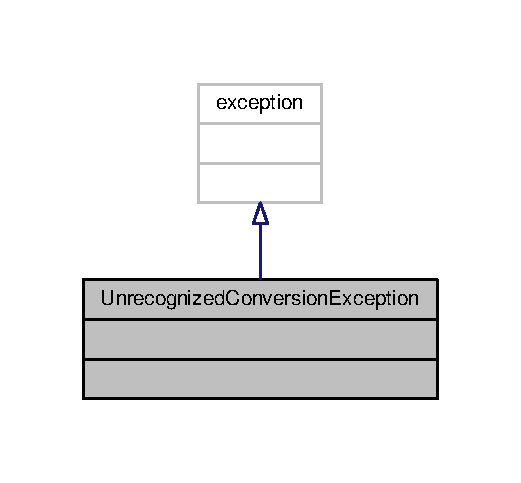
\includegraphics[width=250pt]{class_unrecognized_conversion_exception__inherit__graph}
\end{center}
\end{figure}


Collaboration diagram for Unrecognized\-Conversion\-Exception\-:
\nopagebreak
\begin{figure}[H]
\begin{center}
\leavevmode
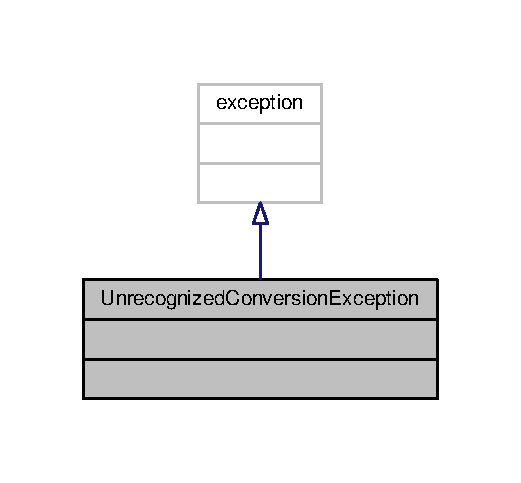
\includegraphics[width=250pt]{class_unrecognized_conversion_exception__coll__graph}
\end{center}
\end{figure}


The documentation for this class was generated from the following file\-:\begin{DoxyCompactItemize}
\item 
characters.\-h\end{DoxyCompactItemize}

\hypertarget{class_world}{\section{World Class Reference}
\label{class_world}\index{World@{World}}
}


Collaboration diagram for World\-:
\nopagebreak
\begin{figure}[H]
\begin{center}
\leavevmode
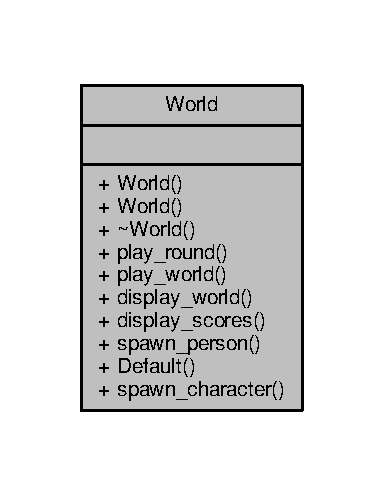
\includegraphics[width=184pt]{class_world__coll__graph}
\end{center}
\end{figure}
\subsection*{Public Member Functions}
\begin{DoxyCompactItemize}
\item 
\hypertarget{class_world_a11cba0453925ea62efa36ba293d9ca18}{{\bfseries World} (Player\-List)}\label{class_world_a11cba0453925ea62efa36ba293d9ca18}

\item 
\hypertarget{class_world_a18a5e578925e7a077b93e689c0f70f18}{{\bfseries World} (unsigned int)}\label{class_world_a18a5e578925e7a077b93e689c0f70f18}

\item 
\hypertarget{class_world_a8027a11b4e3648efebb8daa10f604af1}{void {\bfseries play\-\_\-round} ()}\label{class_world_a8027a11b4e3648efebb8daa10f604af1}

\item 
\hypertarget{class_world_aed8db20661bca96ce422ac52443e94c8}{void {\bfseries play\-\_\-world} ()}\label{class_world_aed8db20661bca96ce422ac52443e94c8}

\item 
\hypertarget{class_world_ac9f7fe8fa51a0053bc4718440ff74a31}{void {\bfseries display\-\_\-world} ()}\label{class_world_ac9f7fe8fa51a0053bc4718440ff74a31}

\item 
\hypertarget{class_world_a0395c6476390f68426ef1a32a204ee4f}{void {\bfseries display\-\_\-scores} ()}\label{class_world_a0395c6476390f68426ef1a32a204ee4f}

\item 
\hypertarget{class_world_a64518dfec673924e6efd0a0fac005b4a}{\hyperlink{class_person}{Person} $\ast$ {\bfseries spawn\-\_\-person} (Player\-Type)}\label{class_world_a64518dfec673924e6efd0a0fac005b4a}

\end{DoxyCompactItemize}
\subsection*{Static Public Member Functions}
\begin{DoxyCompactItemize}
\item 
\hypertarget{class_world_a66d9361da0f0e8bba0c43037a9392744}{static \hyperlink{class_world}{World} {\bfseries Default} ()}\label{class_world_a66d9361da0f0e8bba0c43037a9392744}

\item 
\hypertarget{class_world_a2c923740175b0860080b5aa2859112f5}{static \hyperlink{class_character}{Character} $\ast$ {\bfseries spawn\-\_\-character} (Player\-Type)}\label{class_world_a2c923740175b0860080b5aa2859112f5}

\end{DoxyCompactItemize}


The documentation for this class was generated from the following files\-:\begin{DoxyCompactItemize}
\item 
characters.\-h\item 
characters.\-cpp\item 
world.\-cpp\end{DoxyCompactItemize}

\hypertarget{class_zombie}{\section{Zombie Class Reference}
\label{class_zombie}\index{Zombie@{Zombie}}
}


Inheritance diagram for Zombie\-:
\nopagebreak
\begin{figure}[H]
\begin{center}
\leavevmode
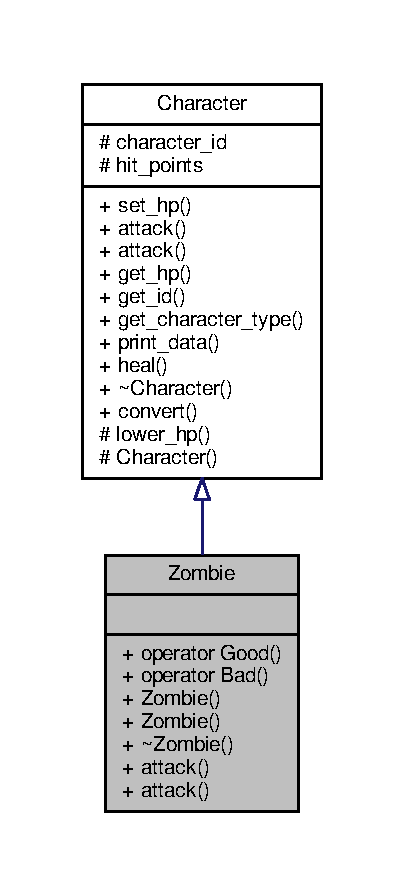
\includegraphics[width=194pt]{class_zombie__inherit__graph}
\end{center}
\end{figure}


Collaboration diagram for Zombie\-:
\nopagebreak
\begin{figure}[H]
\begin{center}
\leavevmode
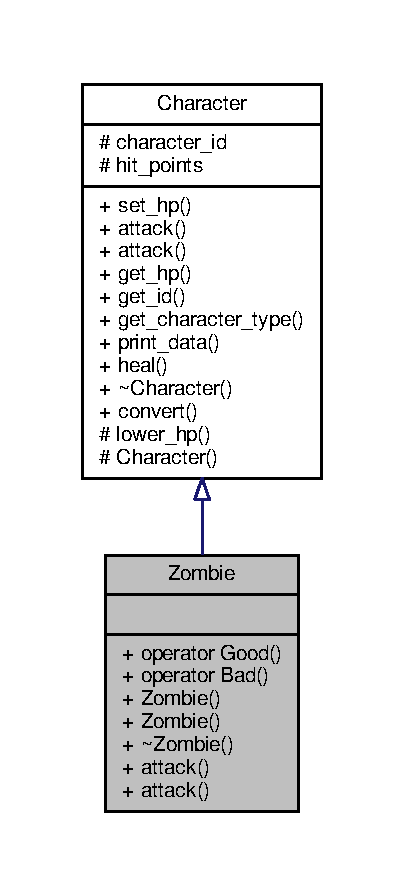
\includegraphics[width=194pt]{class_zombie__coll__graph}
\end{center}
\end{figure}
\subsection*{Public Member Functions}
\begin{DoxyCompactItemize}
\item 
\hyperlink{class_zombie_a6f2a446e7ce66f88e5a7b67b9edf923a}{operator Good} ()
\item 
\hypertarget{class_zombie_ac5c3d335a7876a07b67a87735f643780}{{\bfseries operator Bad} ()}\label{class_zombie_ac5c3d335a7876a07b67a87735f643780}

\item 
\hypertarget{class_zombie_ac56331b5b7d745ddecc375d6f56342d0}{{\bfseries Zombie} (\hyperlink{class_character}{Character} \&)}\label{class_zombie_ac56331b5b7d745ddecc375d6f56342d0}

\item 
\hypertarget{class_zombie_ab0c8072e3ed7c699f3977efc7fd81261}{\hyperlink{class_person}{Person} $\ast$ {\bfseries attack} (\hyperlink{class_person}{Person} \&)}\label{class_zombie_ab0c8072e3ed7c699f3977efc7fd81261}

\item 
\hypertarget{class_zombie_ae6bb1769544b8501b0746a959347cf61}{\hyperlink{class_person}{Person} $\ast$ {\bfseries attack} (\hyperlink{class_person}{Person} $\ast$)}\label{class_zombie_ae6bb1769544b8501b0746a959347cf61}

\end{DoxyCompactItemize}
\subsection*{Additional Inherited Members}


\subsection{Member Function Documentation}
\hypertarget{class_zombie_a6f2a446e7ce66f88e5a7b67b9edf923a}{\index{Zombie@{Zombie}!operator Good@{operator Good}}
\index{operator Good@{operator Good}!Zombie@{Zombie}}
\subsubsection[{operator Good}]{\setlength{\rightskip}{0pt plus 5cm}Zombie\-::operator {\bf Good} (
\begin{DoxyParamCaption}
{}
\end{DoxyParamCaption}
)}}\label{class_zombie_a6f2a446e7ce66f88e5a7b67b9edf923a}
This class inherits from \hyperlink{class_character}{Character} and is used to create Zombies! 

The documentation for this class was generated from the following files\-:\begin{DoxyCompactItemize}
\item 
characters.\-h\item 
characters.\-cpp\end{DoxyCompactItemize}

%--- End generated contents ---

% Index
\newpage
\phantomsection
\addcontentsline{toc}{chapter}{Index}
\printindex

\end{document}
